\documentclass[10pt,a4paper]{article}
\usepackage[utf8]{inputenc}
\usepackage[german]{babel}
\usepackage[T1]{fontenc}
\usepackage{amsmath}
\usepackage{amsfonts}
\usepackage{amssymb}
\usepackage{graphicx}
\begin{document}
\section{Schwebung}
Superposition zweier Schwingungen mit geringem Frequenzunterschied weist periodische Amplitude auf.
\subsection{Herleitung}
2 Schwingungen unterschiedlicher Frequenzen (vereinfachung: gleiche Amplituden) 
\begin{align}
f_1(t)&=A sin(2\pi f_1 t) \notag \\
f_2(t)&=A sin(2\pi f_2 t) \notag \\
f_{Res}(t)&=f_1(t)+f_2(t)=A(sin(2\pi f_1 t)+sin(2\pi f_2 t)) \notag \\
\stackrel{Add. Theorem}{=} 2A\cdot sin(2\pi \underbrace{\frac{|f_1+f_2|}{2}}_{f_Res}t) &\cdot cos(2\pi \underbrace{\frac{|f_1+f_2|}{2}}_{f_{Einhüllende}}t) \notag \\
f_{Schwebung}&=|f_1-f_2|
\end{align}
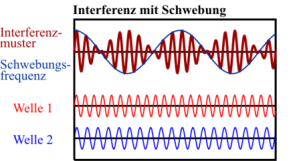
\includegraphics[scale=2]{Interferenz_schwebend.png}\centering
\end{document}